%% Seminar deck: Are Survey-Based Rate Expectations Informative? (WP, 2026)
%% 13 slides, yieldcartography house theme, academic-seminar register.
%% Built from the SSRN working paper. No venue disclosed.
\documentclass[aspectratio=169,11pt]{beamer}
\usepackage{beamerthemeyc}
\renewcommand{\deckfootertitle}{Dec (2026) · Are survey-based rate expectations informative? · SSRN 6644222}

\begin{document}

% 1 ---------------------------------------------------------------------------
\begin{frame}[plain]
  \vspace{2mm}
  {\ttfamily\scriptsize\color{ycmuted}SEMINAR DECK · YIELDCARTOGRAPHY.COM}\\[-0.3em]
  {\color{ycrule}\rule{\textwidth}{0.5pt}}
  \vspace{4mm}

  {\fontsize{19}{23}\selectfont\bfseries\color{ycink}Are survey-based rate expectations\\informative?\par}
  \vspace{2mm}
  {\normalsize\color{ycmuted}Evidence from less-liquid markets.\par}
  \vspace{6mm}
  {\small\bfseries Marcin Dec\par}
  {\footnotesize\color{ycmuted}Kozminski University \& FAME|GRAPE, Warsaw\par}
  \vspace{3mm}
  {\ttfamily\scriptsize\color{ycaccent}Working paper · SSRN 6644222 · doi:10.2139/ssrn.6644222 · under peer review\par}
  \vfill
  \raisebox{-1mm}{
\includegraphics[height=6mm]{kozminski_logo.png}}\hspace{5mm}
  \raisebox{-1mm}{
\includegraphics[height=6mm]{grape_logo.png}}\hspace{5mm}
  \raisebox{-1mm}{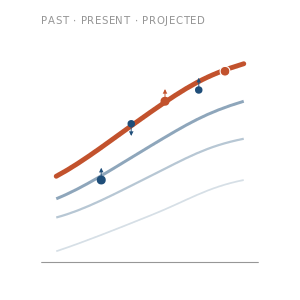
\includegraphics[height=6mm]{yc_logo.png}}
  \hfill{\ttfamily\scriptsize\color{ycmuted}NCN Preludium UMO-2020/37/N/HS4/02202}
\end{frame}

% 2 ---------------------------------------------------------------------------
\begin{frame}{Motivation}
  \kicker{Two expectation measures for one short rate}
  \begin{itemize}
    \item The NBP Survey of Professional Forecasters releases a quarterly
          implied-rate path with annual readings up to five years ahead: the
          closest object the Polish market has to a public consensus
          expected-rate forecast.
    \item The term structure supplies a competing measure: the expected-rate
          path $y^{rf}_t(\tau)$ from the ACM model with the BRW small-sample
          bias correction, fitted on the LW-NSS zero-coupon panel.
    \item The question: \alert{does the survey carry information beyond what
          is already priced into the curve}, and does the answer depend on the
          horizon?
  \end{itemize}
\end{frame}

% 3 ---------------------------------------------------------------------------
\begin{frame}{Data and design}
  \kicker{The horse race}
  \begin{itemize}
    \item Sample: quarterly survey releases 2010Q1--2026Q1; forecast horizons
          $h \in \{12, 24, 36, 48, 60\}$ months.
    \item Realisation: the NBP reference rate observed at each horizon,
          $r_{t+h}$.
    \item Competing forecasts at each release date $t$: the survey path
          $f^{S}_{t,h}$ and the model path $f^{M}_{t,h}$ read off the ACM--BRW
          expected-rate leg at the matching horizon.
    \item Three standard comparisons, run per horizon: Diebold--Mariano on
          squared errors, Clark--West, and Mincer--Zarnowitz forecast
          encompassing.
  \end{itemize}
\end{frame}

% 4 ---------------------------------------------------------------------------
\begin{frame}{Test equations}
  \kicker{Estimating equations and nulls}
  \small With forecast errors $e^{j}_{t,h} = r_{t+h} - f^{j}_{t,h}$,
  $j \in \{S, M\}$:
  \[ d_{t,h} \;=\; \big(e^{M}_{t,h}\big)^2 - \big(e^{S}_{t,h}\big)^2,
     \qquad
     DM_h \;=\; \frac{\bar d_h}{\sqrt{\widehat V_{NW}(\bar d_h)}},
     \qquad H_0\!:\ \mathbb{E}[d_{t,h}]=0 \]
  Clark--West adds the nested-model adjustment term to $d_{t,h}$ before the
  same construction. Forecast encompassing (Mincer--Zarnowitz form):
  \[ r_{t+h} \;=\; c_h + \lambda^{S}_h\, f^{S}_{t,h}
     + \lambda^{M}_h\, f^{M}_{t,h} + \varepsilon_{t+h},
     \qquad H_0\!:\ \lambda^{S}_h = 0 \ \text{(survey encompassed)} \]
  \begin{itemize}
    \item Overlapping $h$-month errors: HAC (Newey--West) variance throughout.
  \end{itemize}
\end{frame}

% 5 ---------------------------------------------------------------------------
\begin{frame}{Headline: relative accuracy by horizon}
  \kicker{MSE(model) / MSE(survey); above 1 the survey wins}
  \begin{center}
  \begin{tikzpicture}[x=1.55cm,y=1.55cm]
    \draw[ycmuted,line width=0.5pt] (0.4,0) -- (0.4,2.1);
    \draw[ycrule,line width=0.4pt] (0.4,0) -- (5.6,0);
    \draw[ycrule,dash pattern=on 2pt off 2pt,line width=0.8pt] (0.4,1) -- (5.6,1);
    \node[right,font=\tiny\itshape,text=ycmuted] at (5.6,1) {parity};
    \foreach \y in {0,1,2} \node[left=2pt,font=\scriptsize,text=ycmuted] at (0.4,\y) {\y.0};
    \foreach [count=\g] \h/\v in {12/1.62, 24/1.21, 36/0.85, 48/0.70, 60/0.62}{
      \pgfmathsetmacro{\xz}{0.65+(\g-1)*1.0}
      \pgfmathparse{\v>1?"ycaccent":"ycsalmon"}
      \fill[\pgfmathresult] (\xz,0) rectangle (\xz+0.6,\v);
      \node[above,font=\scriptsize\bfseries,text=ycink] at (\xz+0.3,\v) {\v};
      \node[below,font=\scriptsize,text=ycmuted] at (\xz+0.3,-0.06) {$h=\h$m};
    }
  \end{tikzpicture}
  \end{center}
  \footnotesize\color{ycmuted} The survey is more accurate at 12 and 24
  months; the model is more accurate from 36 months on, by a widening margin.
  The crossover sits near $h=24$ months.
\end{frame}

% 6 ---------------------------------------------------------------------------
\begin{frame}{Full test results}
  \kicker{DM, CW and encompassing, per horizon}
  \begin{center}
  \small
  \begin{tabular}{rccrrrrl}
    $h$ & MSE$^{M}$ & MSE$^{S}$ & DM & $p$ & CW & $p$ & survey encompassed?\\
    \hline
    12m & 1.42 & 0.88 & $+3.10$ & 0.002 & $+1.85$ & 0.032 & no: survey adds information\\
    24m & 1.69 & 1.40 & $+1.21$ & 0.226 & $+0.55$ & 0.291 & mixed\\
    36m & 1.55 & 1.83 & $-2.04$ & 0.041 & $-1.32$ & 0.094 & yes: survey rejected\\
    48m & 1.30 & 1.85 & $-2.85$ & 0.004 & $-2.11$ & 0.018 & yes\\
    60m & 1.02 & 1.65 & $-3.41$ & 0.001 & $-2.78$ & 0.003 & yes\\
  \end{tabular}
  \end{center}
  \vspace{2mm}
  \footnotesize\color{ycmuted} Positive statistics favour the survey, negative
  favour the model. Realisation: the NBP reference rate. Sample
  2010Q1--2026Q1.
\end{frame}

% 7 ---------------------------------------------------------------------------
\begin{frame}{Result 1: the survey dominates at one year}
  \kicker{The short end of the horizon grid}
  \begin{itemize}
    \item At $h=12$ months the model-to-survey MSE ratio is 1.62
          (MSE 1.42 versus 0.88), with DM $=+3.10$ ($p=0.002$) and CW
          $=+1.85$ ($p=0.032$), both in the survey's favour.
    \item The encompassing regression retains the survey:
          $\lambda^{S}$ is significant at 12 months, so the survey carries
          information beyond the model path.
    \item The information source is timing: respondents observe
          high-frequency news and policy guidance between the model's
          calibration dates.
  \end{itemize}
\end{frame}

% 8 ---------------------------------------------------------------------------
\begin{frame}{Result 2: the model wins from three years on}
  \kicker{The long end of the horizon grid}
  \begin{itemize}
    \item At $h=36$--$60$ months the model's MSE advantage widens (ratios
          0.85, 0.70, 0.62) and is significant on both DM and CW.
    \item Encompassing delivers the strong form: at 36, 48 and 60 months
          $\lambda^{S}$ is indistinguishable from zero while $\lambda^{M}$ is
          not. The model contains the survey's information set and more.
    \item Mechanism: the survey's long-horizon readings are nearly flat,
          anchored on a long-run mean, while the no-arbitrage structure moves
          the model path with the cycle.
  \end{itemize}
\end{frame}

% 9 ---------------------------------------------------------------------------
\begin{frame}{Interpretation}
  \kicker{A horizon division of labour}
  \small
  \begin{itemize}
    \item The two expectation measures exhibit a horizon-specific ordering:
          survey information dominates within one year, the no-arbitrage
          restriction dominates beyond two.
    \item For term-structure work on less-liquid markets, the encompassing
          result justifies using the model path as the expectations benchmark
          at the horizons where term premia are actually estimated, and
          treating long-horizon survey readings as uninformative anchoring.
    \item The one-year result cautions against reading short-run model-survey
          gaps as mispricing; at that horizon the survey is the better-informed
          measure.
  \end{itemize}
\end{frame}

% 10 --------------------------------------------------------------------------
\begin{frame}{Data and econometrics}
  \kicker{Specification summary}
  \small
  \begin{itemize}
    \item \textbf{Survey.} NBP Survey of Professional Forecasters, quarterly
          releases from 2010Q1, implied short-rate path constructed from the
          published annual readings.
    \item \textbf{Model.} ACM affine term-structure model with BRW
          small-sample bias correction on the LW-NSS-fitted Polish zero-coupon
          panel; the expected-rate leg evaluated at the survey's horizons on
          each release date.
    \item \textbf{Inference.} Diebold--Mariano and Clark--West statistics with
          Newey--West variance (overlapping $h$-month errors); encompassing
          regressions estimated per horizon with HAC standard errors.
  \end{itemize}
\end{frame}

% 11 --------------------------------------------------------------------------
\begin{frame}{Companion data and replication}
  \kicker{yieldcartography.com}
  \begin{itemize}
    \item The survey-implied path and the ACM--BRW expected-rate path are
          plotted against each other, release by release, on
          \textcolor{ycaccent}{\ttfamily yieldcartography.com/curves}.
    \item The expected-rate leg updates daily on
          \textcolor{ycaccent}{\ttfamily /term-premia/}; the oracle gauge on
          \textcolor{ycaccent}{\ttfamily /oracle/} reads the same BRW path
          against the professional-forecaster benchmark.
    \item Underlying CSVs are downloadable from the dashboards.
  \end{itemize}
\end{frame}

% 12 --------------------------------------------------------------------------
\begin{frame}[plain]
  \vspace{12mm}
  {\fontsize{27}{31}\selectfont\bfseries\color{ycink}Thank you.\par}
  \vspace{6mm}
  {\normalsize\color{ycink}Marcin Dec\par}
  {\small\color{ycmuted}Kozminski University \& FAME|GRAPE, Warsaw\\
   mdec@kozminski.edu.pl · ORCID 0000-0002-6220-8267\par}
  \vspace{5mm}
  {\ttfamily\footnotesize\color{ycaccent}%
   Dec, M. (2026). Are Survey-Based Rate Expectations Informative?\\
   Evidence from Less-Liquid Markets. SSRN 6644222.\\
   doi:10.2139/ssrn.6644222 · under peer review\par}
  \vspace{5mm}
  {\ttfamily\scriptsize\color{ycmuted}Research supported by the National
   Science Centre, Poland · Preludium UMO-2020/37/N/HS4/02202\par}
  \vfill
  \raisebox{-1mm}{
\includegraphics[height=6mm]{kozminski_logo.png}}\hspace{5mm}
  \raisebox{-1mm}{
\includegraphics[height=6mm]{grape_logo.png}}\hspace{5mm}
  \raisebox{-1mm}{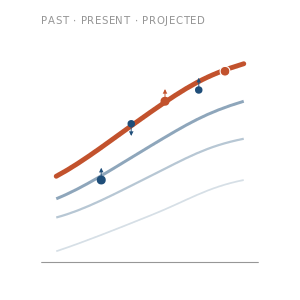
\includegraphics[height=6mm]{yc_logo.png}}
  \hfill{\ttfamily\scriptsize\color{ycmuted}yieldcartography.com/slides/surveys/}
\end{frame}

\end{document}
